% !TeX spellcheck = de_DE
\documentclass{alex_gp}

\name{Alexander Helbok}
\course{Grundpraktikum}
\hwnumber{2}
\spacing{}

\setlength\columnsep{-5cm}
\begin{document}
\renewcommand{\labelenumi}{\alph{enumi})}

\begin{mybox}{Kalibrierung des Rades}
	Das Messgerät wurde von der Tischkante bis zur Wand geschoben und hat währenddessen die Distanz aufgezeichnet. Die zurückgelegte Strecke setzt sich aus dem Abstand zwischen Wand und Tischkante minus der Länge des IOLabs \footnotemark[1] zusammen und wurde auf \\ \( d = 0.665(1) \unit{m} \) gemessen. Die Länge des Tisches wurde an der Kante gemessen, wo man unter Annahme eines rechtwinkeligen Tisches das Lineal äußerst gerade halten kann. Deshalb wurde diese Fehlerquelle nicht miteinbezogen, da sie vernachlässigbar klein ist im Vergleich zum Ablesefehler.\\
	
	\begin{vwcol}[widths={0.3, 0.7}, sep=.8cm, justify=flush,rule=0pt, indent=1em, lines=20] 
		\begin{minipage}[t][0cm][t]{0.3\textwidth}
			\hspace{0.5cm}
			\begin{tabular}{@{} rr @{}}\toprule
				s [m] & a \\ \midrule
				0.661(1) & 0.994(2) \\
				0.663(1) & 0.997(2) \\
				0.663(1) & 0.997(2) \\
				0.664(1) & 0.998(2) \\
				0.662(1) & 0.995(2) \\
				0.662(1) & 0.995(2) \\
				0.661(1) & 0.994(2) \\
				0.660(1) & 0.992(2) \\
				0.664(1) & 0.998(2) \\
				0.665(1) & 1.000(2) \\
				\bottomrule
			\end{tabular}
			\captionof{table}{Gemessene zurückgelegte Strecke \( s \) und die dazugehörige Proportionalitätskonstante \( a \)}
			\label{table:1}
		\end{minipage}%
		\newpage
		\begin{minipage}[t][0cm][t]{0.64\textwidth}
			Der Fehler der Distanzmessung des IOLabs wird bei \( 1 \unit{mm} \) angenommen. Geht man von einem linearen Zusammenhang zwischen der gemessenen Größe und dem berechneten Wert \( f_{\text{gem}} = a f_{\text{calc}} \) erhält man für diese Proportionalitätskonstante 
			\begin{equation}\label{eqn:a0}
					a = \frac{s}{d}
			\end{equation}
			Dies wurde für alle Distanzmessungen (Siehe Tabelle \ref{table:1} gemacht. Aus den 10 Messungen lässt sich der (ungewichtete) Mittelwert \( \bar{a} = 0.99624 \) und die Standardabweichung \( \sigma_a = 0.00212 \) bilden. Der Fehler des Mittelwerts lässt sich wie folgt berechnen
			\begin{equation}\label{eqn:alp}
					\alpha = \frac{\sigma}{\sqrt{N}}
			\end{equation}
			also gilt in unserem Beispiel
			\begin{equation}\label{eqn:afin}
					\bar{a} = 0.9962(7)
			\end{equation}
		\end{minipage}
	\end{vwcol}
	\vspace{-0.5cm}
	Die Standardabweichung \( \sigma_a \) und die Propagierten Fehler für \( a \) in Tabelle \ref{table:1} stimmen auf vier Dezimalstellen überein, die Standardabweichung bietet sich also gut als Abschätzung für den Fehler an, sollte dieser nicht bekannt sein. Sind die Messpunkte nicht Gaußverteilt könnte dieser Ansatz aber nicht mehr stimmen. 
	
	Der Proportionalitätsfaktor \( \bar{a} \) liegt über \( 5 \sigma \) von 1 entfernt, also kann man nicht mehr von einem „gut kalibrierten“ Sensor sprechen. 
	
	Die Richtigkeit des Sensors spiegelt sich in der Abweichung von \( \bar{a} \) vom Optimalwert 1 wieder. Ist \( \bar{a} \) kleiner als 1, wie in unserem Fall, misst der Sensor konstant zu wenig. Dies muss man in der Datenanalyse beachten und berichtigen, indem man alle Messpunkte um den Faktor \( \bar{a} \) skaliert. Wichtig hierbei ist, dass das systematische Abweichungen sind und der hier entstehende Fehler nicht mit dem Statistischen zusammengeworfen werden darf, sondern separat diskutiert werden soll. 
	
	Die Standardabweichung eines Datensatzes ist ein direktes Maß für die Streuung der Punkte und kann daher herangezogen werden, um über die Präzision eines Sensors zu urteilen. Ist die Standardabweichung gering, so streuen die Daten wenig um den Mittelwert, was wiederum für unseren Sensor bedeutet, dass er sehr präzise misst und statistische Schwankungen klein sind. Um die Präzision einer Messung zu verbessern helfen mehr Daten, da jeder Datenpunkt Informationen beinhaltet und daher die Messung/den Fehler der Messung verbessert.
	
	\footnotetext[1]{https://www.macmillanlearning.com/college/us/digital/iolab/technical-specs}
\end{mybox}

\begin{mybox}{Bemessung von \( g \)}
	Um die Erdbeschleunigung \( g \) zu messen, wurde ein Pendel mit einem Kraftsensor ausgestattet. Die Länge \( L \) des Pendels besteht aus der Fadenlänge, an welchem das IOLab befestigt ist, und der Distanz von Aufhängepunkt am Messgerät bis zu dessen Massezentrum. Der Schwerpunkt des IOLabs ist mit einem \( 4\times 4 \unit{mm} \) Kasten markiert. Letztere Distanz wurde mit einer elektronischen Schublehre von der Kante bis zum Mittelpunkt der Box gemessen; die prominente Unsicherheit kommt hier aus der wagen Kennzeichnung des Schwerpunkts und wurde auf \( 2 \unit{mm} \) geschätzt. Der Fehler der Fadenlänge beträgt auch \( 2 \unit{mm} \). Hierbei wurde der Ablesefehler, die Krümmung des Maßbandes und die Lokalisierung der Drehachse berücksichtigt. Die Gesamtlänge beträgt 
	\begin{equation}
		L = 0.538(3) \unit{m}
	\end{equation}
	Die Periodendauer \( T_0 \) des mathematische Pendels wird unter Annahme der Kleinwinkelnäherung durch 
	\begin{equation}\label{eqn:T0}
		T_0 = 2\pi\sqrt{\tfrac{L}{g}}
	\end{equation}
	beschrieben, wobei \( g \) die Gravitationsbeschleunigung auf der Erde darstellt. Um die Periodendauer mithilfe der Daten des Kraftsensors zu bestimmen wurde eine Sinuskurve der Form \( A * \sin(\omega x + \varphi) + k \) an die Messpunkte angepasst. Der Fitprozess verlief in drei Schritten.
	
	Da die Daten sehr verrauscht waren mussten sie zuerst geglättet werden. Danach wurde ein Sinus in der allgemeinen Form mit vier freien Parametern an die Daten von \( t = 4 \unit{s} \) bis \( t = 5 \unit{s} \) angepasst. Im dritten Schritt wurde wieder ein Sinus mit zwei freien Variablen (\( \omega, \varphi \)) an den Zeitraum von zwei bis sieben Sekunden gefittet, wobei \( A \) und \( k \) auf den im zweiten Schritt ermittelten Werten festgehalten wurden. 
	
	Das Ergebnis ist in Abbildung \ref{fig:sine} dargestellt und liefert eine Periode von
	\begin{equation}\label{eqn:period}
		T_0 = 2 \frac{2\pi}{\omega} = 1.4955(3) \unit{s}
	\end{equation}
	Hier darf man den Faktor 2 nicht vergessen, der daher stammt, dass die Kraft auf den Sensor des Pendels bezüglich der Senkrechten symmetrisch ist und in einer Periode zwei Maxima (Ruhelage) und zwei Minima (maximale Auslenkung) durchlaufen werden.
	\begin{figure}[H]
		\vspace{-0.5cm}		
		\centering
		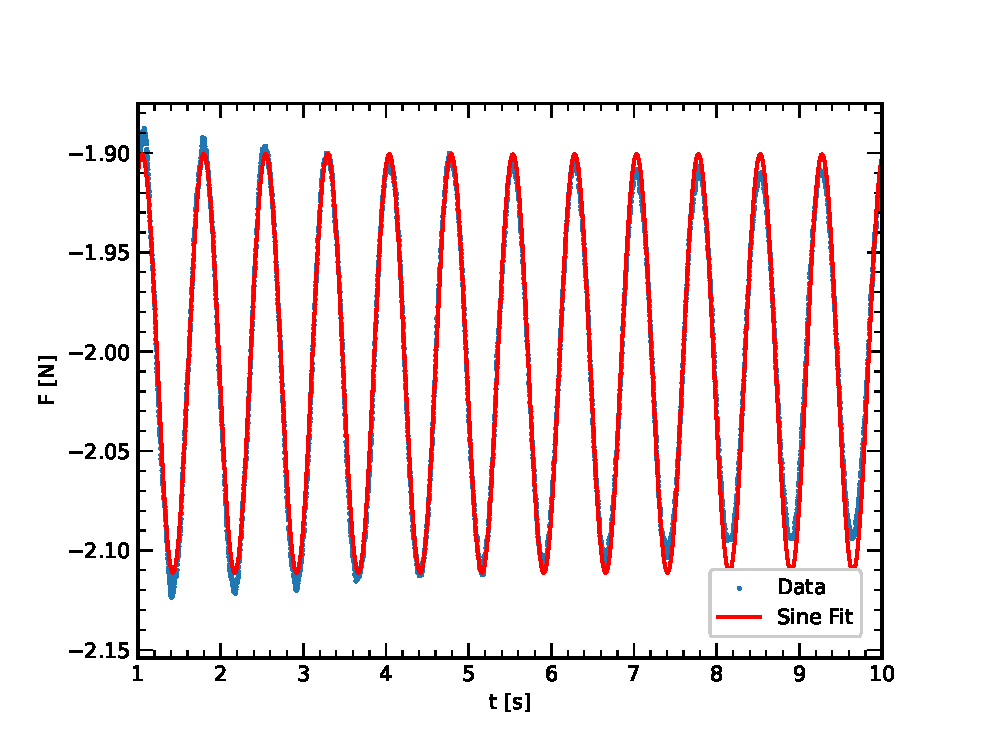
\includegraphics[width=\textwidth]{Versuch2_1.eps}
		\caption{Beschönigte Daten des Kraftsensors während der ersten 12 „schönen“ Schwingungen des Pendelvorgangs. Eine Sinuskurve wurde in den Zeitraum von 2 bis 7 Sekunden angepasst.}
		\label{fig:sine}
	\end{figure}
	Setzt man die ermittelten Werte in Gleichung \ref{eqn:T0} ein erhält man
	\begin{equation}\label{eqn:g0}
		g = 4\pi^2 \frac{L}{T_0^2} = 9.50(5) \unit{\a}
	\end{equation}
	Dieser Wert weicht fast \( 10\sigma \) vom Literaturwert und ist daher nicht mit ihm vereinbar, was aber nicht heißt, dass hier neue Physik geschieht und eine Entdeckung gefeiert werden kann. Der Kraftsensor wurde noch nicht Kalibriert also könnte es sein, dass das Messgerät systematisch zu niedrig misst. Des Weiteren wurden weder Luftwiderstand noch Reibung berücksichtigt und die Kleinwinkelnäherung wurde getroffen, was aber dieses Resultat nicht alleine beschreiben können. 
	
	Gleichung \ref{eqn:T0} macht Gebrauch der Kleinwinkelnäherung und weicht daher von der exakten Lösung ab. Will man der analytischen Lösung näher kommen kann man Terme aus der Taylorentwicklung der genäherten Winkelfunktionen einbauen und erhält dann
	\begin{equation}\label{eqn:T2}
		T_2 = \left(1 + \tfrac{\theta_0^2}{16}\right) T_0 = 2\pi\left(1 + \tfrac{\theta_0^2}{16}\right)\sqrt{\tfrac{L}{g}}
	\end{equation}
	\( \theta_0 \) beschreibt hier die maximale Auslenkung des Pendels und kann mithilfe einer zweiten Messung in Ruhelage bestimmt werden. Die Kraft in Ruhelage beträgt \( F_0 = mg = -1.97095(1) \unit{N} \) und wurde als ungewichteter Mittelwert einer 30 Sekunden langen Messung berechnet. Die Kraft beim Winkel \( \theta_0 \) ist gerade \( F(\theta_0) = mg\cos(\theta_0) = -1.90069(6) \unit{N} \) und ist die Summe der Amplitude \( A \) und der Vertikalverschiebung \( k \) aus dem Sinusfit. \( \theta_0 \) lässt sich also wie folgt schreiben
	\begin{equation}\label{eqn:theta}
		\theta_0 = \arccos(\frac{F(\theta_0)}{F_0}) = \ang{15.344(7)}
	\end{equation}
	Jetzt kann man Werte in \ref{eqn:T2} einsetzen und erhält
	\begin{equation}\label{eqn:g1}
		g = 4\pi^2 \frac{L}{T_0^2}\frac{1}{\left(1 + \tfrac{\theta_0^2}{16}\right)} = 9.45(5) \unit{\a}
	\end{equation}
	Dieser Wert liegt noch innerhalb des \( 1\sigma \) Fehlers von \ref{eqn:g0} und könnte daher auch gut durch reine statistische Schwankungen zustande kommen. Die Verwendung eines genaueren Ausdrucks verbessert das Messergebnis nicht drastisch. 
	
	Wenn man die einzelnen Beiträge im Fehler von \( g \) betrachtet bemerkt man, dass die aus dem Fit bestimmten Periode nur \( \approx 0.5 \unit{\percent} \) zum Gesamtfehler beiträgt, während die Bestimmung der Fadenlänge und des Schwerpunkts jeweils über \( 49 \unit{\percent} \) ausmachen. 
\end{mybox}

\begin{mybox}{Kalibrierung des Kraftsensors}
	\begin{vwcol}[widths={0.6,0.4}, sep=.8cm, justify=flush,rule=0pt, indent=1em, lines=21] 
		Um die Präzision und Richtigkeit des Kraftsensors zu eruieren wurde eine Probemasse in Form von Münzen an den Sensor gehängt und den gemessen Wert mit dem Berechneten verglichen. Anzahl und Masse der verwendeten Münzen bitte Tabelle \ref{table:2} entnehmen.
		
		Es wurden für \( 10 \unit{s} \) Daten vom  Kraftsensor aufgezeichnet und davon der ungewichtete Mittelwert berechnet. Die gemessene Kraft 
		\begin{equation}\label{eqn:Fgem}
			F_{\text{gem}} = -0.394 \unit{N}
		\end{equation}
		wird mit drei signifikanten Stellen angegeben, um mit denen des berechneten Werts übereinzustimmen.
		Die Angabe der Kraft erfolgt hier ohne Fehler, weil der Standardfehler so gering ist (da in den \( 10 \unit{s} \) fast 30.000 Datenpunkte gesammelt wurden).
		\newpage
		\begin{minipage}[t][1cm][t]{0.35\textwidth}
			\begin{tabular}{@{} rrr @{}}\toprule
				Wert & Anzahl & Masse [g] \\ \midrule
				1 Cent & 2 & 2.30(2) \\
				2 Cent & 7 & 3.06(3) \\
				5 Cent & 3 & 3.92(4) \\
				10 Cent & 1 & 4.10(4) \\
				20 Cent & 0 & 5.74(6) \\
				50 Cent & 0 & 7.80(8) \\
				1 Euro & 0 & 7.50(8) \\
				2 Euro & 0 & 8.50(9) \\
				\midrule
				\( \sum \) & 13 & 41.9(3) \\
				\bottomrule
			\end{tabular}
			\captionof{table}{Anzahl der verwendeten Münzen und deren Einzelgewicht.}
			\label{table:2}
		\end{minipage}
	\end{vwcol}
	\vspace{-2cm}\noindent
	Verwendet man nun die Erdbeschleunigung aus \ref{eqn:g0} und berechnet damit die Kraft erhält man
	\begin{equation}\label{eqn:Ferr}
		F_{\text{calc}} = -mg = -0.398(3) \unit{N}
	\end{equation}
	was zu einer Proportionalitätskonstante von 
	\begin{equation}\label{eqn:a1}
		a = \frac{F_{\text{gem}}}{F_{\text{calc}}} = 0.991(8)
	\end{equation}
	führt. Dieses Resultat kann man weiter Verbessern, indem man den für \( g \) dem Wert aus \ref{eqn:g1} einsetzt. Dies liefert
	\begin{equation}\label{eqn:a2}
		F_{\text{calc}} = -0.396(3) \unit{N} \quad \text{und} \quad  a = 0.995(8)
	\end{equation}
	Die Abweichung vom Optimalwert 1 kann durch reine statistische Schwankungen erklärt werden. Setzt man für \( g \) aber 9.806 \footnote{https://www.ptb.de/cms/fileadmin/internet/fachabteilungen/abteilung\_1/1.1\_masse/1.15/gravzonen.pdf} ein  erhält man \( a = 0.960(6) \). Der Kraftsensor weicht also systematisch vom Literaturwert ab, was auch die zu niedrigen Werte für \( g \) aus \ref{eqn:g0} und \ref{eqn:g1} erklärt. Korrigiert man nachträglich \ref{eqn:g1} erhält man \( g = 9.85(8) \unit{\a} \) was sich gut mit den Literaturwert vereinbaren lässt. \par
	
	Führt man nun in Zukunft Messungen mit dem Kraftsensor durch, sollte man unter Verwendung des berechneten Proportionalitätsfaktor die Daten berichtigen und das auch im Text erwähnen. Eine möglichst genaue Konstante ist hier von Vorteil und um den Fehler in \( a \) klein zu halten, muss man die verwendete Probemasse sehr genau kennen. In unserem Beispiel könnte man den Fehler reduzieren, indem man möglichst viele kleine/leichte Münzen nimmt. Das erkennt man daran, dass der Standardfehler und der relative Fehler gegeben sind durch
	\begin{equation}\label{eqn:alpha}
		\alpha = \frac{\sigma}{\sqrt{N}} = \frac{0.01\mu}{\sqrt{N}}
	\end{equation}
	und
	\begin{equation}\label{eqn:relalpha}
		\alpha_{\text{rel}} = \frac{\alpha}{\mu} = \frac{0.01}{\sqrt{N}} = \frac{1}{100\sqrt{N}}
	\end{equation}
	Will man den Fehler reduzieren, muss man die Anzahl \( N \) erhöhen, was in unserem Fall bedeutet, eine Gesamtmasse von zb. \( 100 \unit{g} \) aus vielen Leichten (am Besten 43 Stück 1 Cent Münzen) anstatt wenigen Schweren zusammenzustellen.
\end{mybox}


\end{document}